\documentclass[a4paper,10pt]{article}
\usepackage[paperwidth=210mm, paperheight=297mm, left=2.5cm, top=2.5cm, right=2.5cm, bottom=1.0cm, head=1.5cm, includefoot]{geometry}
%\usepackage[latin1]{inputenc}
\usepackage[utf8]{inputenc}
\usepackage[spanish,activeacute]{babel}
\usepackage{bookman}
\usepackage{booktabs}
\usepackage[pdfborder={0 0 0}]{hyperref}
\usepackage{pdfpages}
\usepackage{fancyhdr}
\usepackage{lastpage}
\usepackage{verbatim}
\usepackage{graphicx}
\usepackage{fixltx2e}
\usepackage{listings}

%\usepackage[T1]{fontenc}
%\usepackage{comment}
%\usepackage{makeidx}
%\usepackage{float}
%\usepackage{slashbox}

\renewcommand{\headrulewidth}{1pt}
\renewcommand{\footrulewidth}{1pt}



%%%%%%%%%  Datos  %%%%%%%%%

\title{ \textbf{Trabajo pr\'actico 0: Infraestructura b\'asica } }

\author{Contini, Agust\'in - \textit{Padr\'on 89180}			\\
            \texttt{ agscontini@gmail.com }				\\
            Farina, Federico - \textit{Padr\'on 90177}			\\
            \texttt{ federicojosefarina@gmail.com }				\\
            Prystupiuk, Maximiliano  - \textit{Padr\'on 94  }			\\
            \texttt{ mprystupiuk@gmail.com  }					\\[2.5ex]
            1er. Cuatrimestre de 2017					\\[1.0ex]
            \normalsize{66.20 Organizaci\'on de Computadoras}		\\
            \normalsize{Facultad de Ingenier\'ia, Universidad de Buenos Aires}	\\
	}
\date{\today}

%%%%%%%%%  Fin datos  %%%%%%%%%



\begin{document}



%%%%%%%%%  1era hoja: caratula y datos  %%%%%%%%%

\maketitle
\bigskip
\thispagestyle{empty}	% quita el numero en la primera pagina

\begin{abstract}
El trabajo práctico consiste en implementar el algoritmo de ordenamiento Quicksort y BubbleSort en lenguaje C, las funciones swap y compare, para luego comparar sus respectivas performance y la cantidad de llamados a swap y compare.
\end{abstract}

%%%%%%%%%  Fin 1era hoja  %%%%%%%%%



%%%%%%%%%  Head y foot  %%%%%%%%%

\pagestyle{fancy}
\lhead{
\includegraphics[width=1.2cm]{./img/logo.png}}
\chead{Trabajo pr\'actico 0: Infraestructura b\'asica \\ \textit{Contini  -  Farina  -  Prystupiuk} }

\rfoot{$1^{er}$ Cuatrimestre 2017}
\lfoot{66.20 Organizaci\'on de Computadoras}
\cfoot{\hspace{2.4cm}   P\'agina \thepage \, de \pageref{LastPage} }

%%%%%%%%%  Fin head y foot  %%%%%%%%%



\normalsize

\newpage
\tableofcontents	% hoja de indices de titulos, subtitulos

\vspace{2.0cm}
\listoffigures		% hoja de indices de figuras



\newpage
\section{Introducci\'on}

\subsection{Bubblesort}
El Bubblesort es un algoritmo de ordenamiento que funciona revisando cada elemento de la lista que va a ser ordenada con el siguiente, intercambi\'andolos de posici\'on si est\'an en el orden equivocado. Es necesario revisar varias veces toda la lista hasta que no se necesiten m\'as intercambios, lo cual significa que la lista est\'a ordenada. Dado que s\'olo usa comparaciones para operar elementos, se lo considera un algoritmo de comparaci\'on, siendo el m\'as sencillo de implementar.

\subsection{Quicksort}
 Se elige un elemento de la lista de elementos a ordenar, al que llamaremos pivote. Resituar los dem\'as elementos de la lista a cada lado del pivote, de manera que a un lado queden todos los menores que \'el, y al otro los mayores. Los elementos iguales al pivote pueden ser colocados tanto a su derecha como a su izquierda, dependiendo de la implementación deseada. En este momento, el pivote ocupa exactamente el lugar que le corresponderá en la lista ordenada. La lista queda separada en dos sublistas, una formada por los elementos a la izquierda del pivote, y otra por los elementos a su derecha. Se repite este proceso de forma recursiva para cada sublista mientras \'estas contengan m\'as de un elemento. Una vez terminado este proceso todos los elementos estar\'an ordenados. Como se puede suponer, la eficiencia del algoritmo depende de la posición en la que termine el pivote elegido.En el mejor caso, el pivote termina en el centro de la lista, dividi\'endola en dos sublistas de igual tamaño. En este caso, el orden de complejidad del algoritmo es O(n·log n). En el peor caso, el pivote termina en un extremo de la lista. El orden de complejidad del algoritmo es entonces de O(n\textsuperscript{2}). El peor caso dependerá de la implementación del algoritmo, aunque habitualmente ocurre en listas que se encuentran ordenadas, o casi ordenadas. Pero principalmente depende del pivote, si por ejemplo el algoritmo implementado toma como pivote siempre el primer elemento del array, y el array que le pasamos est\'a ordenado, siempre va a generar a su izquierda un array vac\'io, lo que es ineficiente. En el caso promedio, el orden es O(n·log n). No es extraño, pues, que la mayor\'ia de optimizaciones que se aplican al algoritmo se centren en la elecci\'on del pivote.



\newpage
\section{El programa}

\subsection{Compilado}
Se incluye junto a este trabajo un Makefile para compilar el programa. Simplemente debe abrirse una Terminal en el directorio root. Poner "mkdir build", "cd build", "cmake ..", "make".

\subsection{Uso}
El programa puede leer tanto datos desde stdin como de archivos pasados por par\'ametro. La salida del programa es por stdout y la de errores por stderr.
Forma de uso:
\begin{verbatim}
Usage:
  ./tp0 -h
  ./tp0 -V
./tp0 [OPTIONS] [file...]
  -h, --help       Print this and exit.
  -V, --version    Print version and exit.
  -o, --output     Path to output file.
  -i, --input      Path to input file.
  -b, --bsort      Use bubblesort.
  -q, --qsort      Use quicksort.
\end{verbatim}



\newpage
\section{Desarrollo}

\subsection{Estructura interna del programa}
Se desarrollaron los algoritmos con vistas a cumplir el objetivo del programa. A continuaci\'on se realiza una descripci\'on de cada uno:
\begin{itemize}
	\item 1. Se detectan los argumentos de entrada por l\'inea de comandos, mediante una comparaci\'on de caracteres.
	\item 2. Para los argumentos help y Version, se imprimen cadenas de texto con la informaci\'on b\'asica de uso, y de la versi\'on e integrantes del trabajo.
	\item 3. Para los argumentos Bubblesort y Quicksort, se siguen una serie de pasos:
	\begin{itemize}
		\item a) Si se detectan m\'as argumentos de entrada, se lo utiliza como archivos de entrada. En caso contrario, se abre la entrada est\'andar stdin.
		\item b) Se abren los archivos de entrada en el orden de la l\'inea de comandos y se realiza un ciclo sobre cada uno de ellos, hasta el fin de archivo. En dicho ciclo se realiza un parseo del archivo y se almacena cada palabra en un vector com\'un para todos los archivos. Este vector trabaja con memoria din\'amica.
		\item c) Luego de procesar todos los archivos se llama al ordenamiento pedido por par\'ametro.
		\item d) Luego se procede a imprimir por la salida est\'andar stdout. Se imprime palabra por palabra, recorriendo el vector ya ordenado.
		\item e) Por \'ultimo, se libera la memoria pedida.
	\end{itemize}
\end{itemize}


\bigskip
\subsection{Aclaraciones}
La raz\'on por la cual decidimos hacer una versi\'on corrida para Linux y otra para Gxemul es para poder tener tiempos comparables. Para los speedups, decidimos correr las pruebas de tiempos de Bubblesort y Quicksort en C en Linux y en Gxemul. Para que los tiempos para las comparaciones y speedups fueran comparables, cada sort para cada texto a comparar fueron corridas en ambos sistemas operativos.



\newpage
\subsection{Mediciones de tiempo de ejecuci\'on}
\subsubsection{Resultado de las ejecuciones}

\begin{figure}[h!]
	\centering
	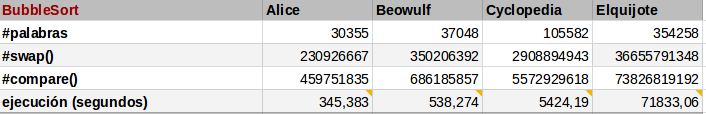
\includegraphics[scale=0.7]{./recursos/bubblesort.png}
	\caption{Tabla de los tiempos del algoritmo de ordenamiento bubblesort}
\end{figure}

\begin{figure}[h!]
	\centering
	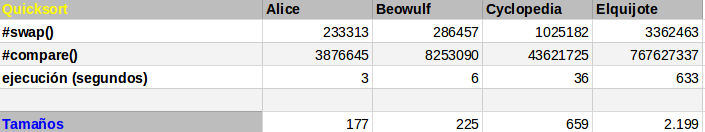
\includegraphics[scale=0.7]{./recursos/quicksort.png}
	\caption{Tabla de los tiempos del algoritmo de ordenamiento quicksort}
\end{figure}


\subsubsection{Gr\'aficos comparando los swaps de los sort}

\begin{figure}[h!]
	\centering
	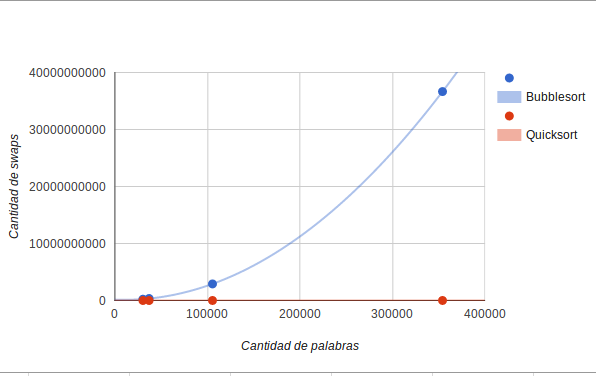
\includegraphics[scale=0.7]{./recursos/swapVsPala.png}
	\caption{Gr\'afico comparando la cantidad de swaps de los sorts corridos en Linux}
\end{figure}

\subsubsection{Gr\'aficos comparando los compare de los sort}

\begin{figure}[h!]
	\centering
	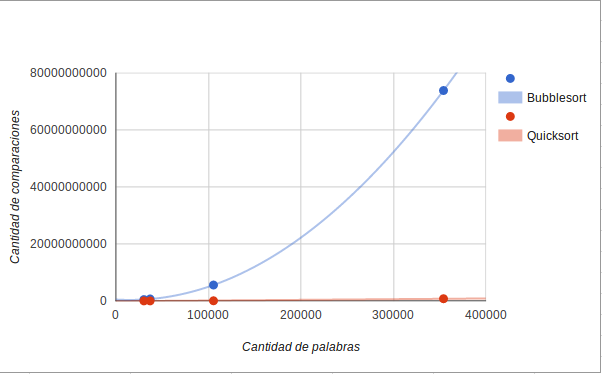
\includegraphics[scale=0.7]{./recursos/compareVsPala.png}
	\caption{Gr\'afico comparando la cantidad de compare de los sorts corridos en Linux}
\end{figure}

\bigskip
Como podemos apreciar, con escala lineal para el eje y (tiempo tardado del sort), por la abismal diferencia entre el Bubblesort y Quicksort, \'esta \'ultima no posee pendiente. As\'i que presentamos el mismo gr\'afico, pero con escala logar\'itmica en el eje y, para poder ver mejor las diferencias.

\subsubsection{Gr\'aficos comparando los tiempos de los sort por palabras}

\begin{figure}[h!]
	\centering
	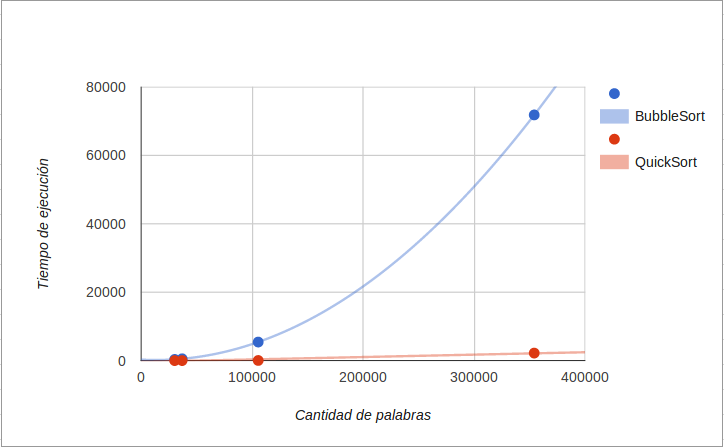
\includegraphics[scale=0.7]{./recursos/ejecVsPala.png}
	\caption{Gr\'afico comparando la cantidad de tiempo de los sorts corridos en Linux por palabras del documento}
\end{figure}


\newpage
\bigskip
Podemos observar que a medida que el tamaño de los archivos aumenta, el Bubblesort tarda cada vez más en ordenar las palabras, mientras que el Quicksort tiene una pendiente menos pronunciada. Esto se debe a las características inherentes de los algoritmos. El Bubblesort no es un algoritmo eficiente ya que realiza muchas comparaciones innecesarias al no presentar un procedimiento que aproveche las comparaciones ya realizadas. Esto hace que se vuelva muy lento, lo cual se acent\'ua cuanto mayor es el n\'umero de palabras a ordenar.

Para el caso del algoritmo Quicksort implementado en C se puede observar que es ampliamente superior al Bubblesort y que el tiempo demorado es muy inferior en ambos ssoo. El compilador de C, al estar ya optimizado para pasar del lenguaje C a assembler, realiza la menor cantidad de accesos a memoria posible y así haciendo, en nuestro caso, el algoritmo de ordenamiento más óptimo.

La cantidad de llamados a compare y swap entre ambos algoritmos es muy marcada, dando esto un claro indicio del porque de la diferencia en los tiempos de ejecuci\'on en cada caso.



\newpage
\subsubsection{C\'alculo del Speedup}
El speedup es una relaci\'on entre el tiempo mejorado y el tiempo anterior a la mejora de, en nuestro caso, una aplicaci\'on. Este valor nos dar\'a una idea de cu\'anto m\'as r\'apido realiza una rutina un programa respecto de otro (en nuestro caso, Bubblesort contra Quicksort).

La f\'ormula para calcularlo es la siguiente:
\begin{center}
	\scalebox{1.8}{ $ SpeedUp = \frac {T_{original}} {T_{mejorado}} $ }
\end{center}

\medskip
En nuestro caso:

\begin{center}
	\scalebox{1.8}{ $ SpeedUp = \frac {T_{bubblesort}} {T_{quicksort}} $ }
\end{center}


\bigskip
Reemplazando con los datos antes mencionados:

\begin{figure}[h!]
	\centering
	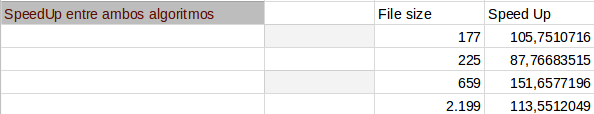
\includegraphics[scale=0.7]{./recursos/SpeedUpAlgoritmos.png}
	\caption{Tabla de los speedups obtenidos de los sorts}
\end{figure}

\bigskip
Pasamos los datos antes calculados a un gr\'afico para observar mejor c\'omo evoluciona el Speedup.
\begin{figure}[h!]
	\centering
	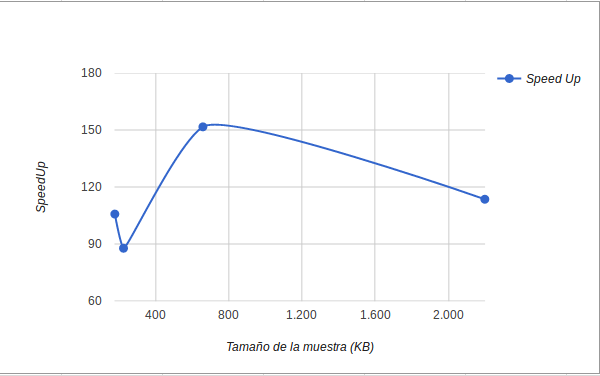
\includegraphics[scale=0.7]{./recursos/speedUpMuestra.png}
	\caption{Gr\'afico del speedup entre Bubblsort en C y Quicksort en C}
\end{figure}

\bigskip
A medida que el tamaño del archivo aumenta, el Speedup del Quicksort respecto del Bubblesort también aumenta. Esto es debido al comportamiento de los algoritmos a la hora de ordenar los archivos. Como se vio en la sección anterior, cuanto más grande es la cantidad de palabras del archivo, el Bubblesort tarda mucho más que el Quicksort. Por lo tanto, viendo la fórmula del Speedup, la relación de los tiempos cada vez va aumentando, haciendo que aumente el Speedup.



\newpage
\section{Conclusiones}
En el presente trabajo se analizó el comportamiento del ordenamiento de archivos de distintos tamaños con los algoritmos Bubblesort y Quicksort. Se pudo observar que el ordenamiento del Quicksort es más rápido que el del Bubblesort. En las sucesivas mediciones se pudo comprobar que a medida que aumentaba el tamaño del archivo a ordenar el Bubblesort realizaba el ordenamiento considerablemente más lento que el otro algoritmo.

Los posteriores cálculos de los Speedups permitieron dar una idea más concisa sobre la mejora de un algoritmo respecto de otro.



\newpage
\section{C\'odigo}

\subsection{sorters.h}
\lstset{ language = C, numbers=left, tabsize=4, breaklines=true, frame=single }
\lstinputlisting{./sorters.h}

\bigskip
\subsection{sorters.c}
\lstset{ language = C, numbers=left, tabsize=4, breaklines=true, frame=single }
\lstinputlisting{./sorters.c}

\bigskip
\subsection{main.c}
\lstset{ language = C, numbers=left, tabsize=4, breaklines=true, frame=single }
\lstinputlisting{./main.c}



\end{document}
